
% { \color{gray}

% \lin


% \cite{FioreTheCase2020}
% -- Coherent states are, apparently, crucial if we want these spaces to have applications

% -- The weak system of coherent states $\mathcal W^d$ is made of the states minimizing $(\Delta \vec x)^2$: they are related to the diagonalization of the coordinates $x_i$; they are $O(D)$-invariant.

% -- A class of $O(D)$-invariant strong SCS are introduced, and in particular an interesting one is $\mathcal S^d$ which minimizes, within this class of CS, $(\Delta \vec x)^2$

% -- The diagonalization of the position observables seems to be improved on their last paper

% \lin

% }


As previously mentioned in the introduction, coherent states of an algebraic space associated to a Hilbert space \todo{Asegurarme de hablar de la importancia de estados coherentes en la introduccion!} are concrete objects with defined properties that enable the application of these spaces. In this chapter we describe some families of coherent states on the new fuzzy circle $S^1_\Lambda$ following \cite{FioreCoherent2020, FioreXi2020, FioreTheCase2020}, and study their localization properties for both position and angular momentum. 

Coherent states are vectors of the underlying Hilbert spaces, and so they induce states of the algebra. Our purpose will be to eventually study the distance between the family of states described in this document.

Throughout this chapter let $\hcal_\Lambda$ and $\acal_\Lambda$ be defined as in definition \ref{definitionHLambdaALambdaD2} for some $\Lambda \in \NN$ and some appropriate function $k = k(\Lambda)$ satisfying the inequality \eqref{inequationInequalityNeededforKasFunctionLambdaD2}, where $\{\psi_m\}_{|m| \leq \Lambda}$ given in \eqref{equationDefinitionPsimD2BasisOfHCutE} are an orthonormal basis of $\hcal_\Lambda$ composed of eigenvalues of $\cut L \in \acal_\Lambda$. Additionally, let the operators $\cut L$ and $\chi^\pm \in \acal_\Lambda$ be defined as in section \ref{chNewFuzzySectionObservables}, but let us use the symbol $L$ instead of $\cut L$. We will call $L$ the angular momentum observable and $\chi^1 = \frac{1}{2}(\chi^+ + \chi^-)$ and $\chi^2 = \frac{1}{2i}(\chi^+ - \chi^-)$ the position observables.

% \section{Localization}
% %%%%%%%%%%%%%%%%%%%%%%%%%%%%%%%%%%%%%%%%%%%%%%%%%%%%%%%%%
Given vector $\psi \in \hcal_\Lambda$, we will use the following measure of the localization of the vector in configuration space:
\begin{equation}
    (\Delta \vec x)^2 = \sum_{i = 1}^D (\Delta x^i)^2 = \langle (\vec x - \langle \vec x \rangle)^2 \rangle = \langle \vec x^2 \rangle - \langle \vec x \rangle ^2,
\end{equation}
where the expectation value for any observable $A$ is
\begin{equation}
    \langle A \rangle = \langle \psi | A | \psi \rangle.
\end{equation}

Similarly, for localization on momentum space the measure will be:
\begin{equation}
    (\Delta \cut L)^2 = \langle (\cut L - \langle L \rangle )^2 \rangle = \langle L^2 \rangle - \langle L \rangle ^2;
\end{equation}
from now on we will denote $\cut L \in \acal_{\Lambda}$ simply by $L$.

\section{Angular Momentum Saturating Coherent States}
%%%%%%%%%%%%%%%%%%%%%%%%%%%%%%%%%%%%%%%%%%%%%%%%%%%%%%%%%

The orthonormal basis $\{\psi_m\}_{|m| \leq \Lambda}$ is our first family of coherent states. 

The group 
\begin{equation}
    G = \{S^n e^{i(aL + b)} \,:\, (a, b, n) \in \RR^2 \times \ZZ_{2\Lambda + 1}\} \cong U(1) \times U(1) \rtimes \ZZ_{2\Lambda + 1}
\end{equation}
where $S$ is the ladder operator defined in \ref{definitionLadderOperatorsHLambda}, with operation
\begin{equation*}
    S^n e^{i(aL+b)}\, S^{n'}e^{i(a'L+b')} = S^{n + n'} e^{i[(a+a')L + (b + b' + an')]},
\end{equation*}
acts unitarily, transitively and irreducibly on $\{\psi_m\}_{|m|\Lambda}$, and the isotropy subgroup $H$ of all $\psi_m$ under this group action is clearly
\begin{equation}
    H = \{e^{i(aL+b)} \,:\, (a, b) \in \RR^2 \} \cong [U(1)]^2.
\end{equation}
Hence 
\begin{equation}
    G/H = \{S^n \,:\, n \in \ZZ_{2\Lambda + 1}\} \cong \ZZ_{2\Lambda + 1},
\end{equation}
is the label space for the basis $\{\psi_m\}_{|m|\leq \Lambda}$. \todo{Do they maximize the isotropy subgroup? Is there an uncertainty relation, perhaps related to the Casimir (is this a Lie group? Semisimple?), that is minimized by this system of coherent states?}

Additionally, the fact that they are a basis means that we have the resolution of the identity
\begin{eqnsplit}\label{resolutionIdentityPsimHcalLambda}
    1_{\hcal_\Lambda} &= \sum_{ m = -\Lambda}^\Lambda \tilde P_m \\
    &= \int_{G/H} \tilde P_m \, d\mu(m),
\end{eqnsplit}
where $\mu$ is the counting measure on $G/H$, induced by the Haar measure on the Lie group $G$. Hence $\{\psi_m\}_{|m| \leq \Lambda}$ is a strong system of coherent states \ref{definitionSystemCoherentStates}.

Now, let's study the localization of these vectors. Since each $\psi_m$ is an eigenvalue of $L$, $(L - \langle L\rangle ) \psi_m = 0$, 
\begin{equation}
    (\Delta L)^2 = 0.
\end{equation}
Similarly, $\langle \psi_m | \chi^i | \psi_m \rangle = 0$, so. $\langle \chi^i \rangle = 0$ for each $i = 1, 2$, and therefore $(\Delta \chi^i)^2 = \langle (\chi^i)^2 \rangle$, and so
\begin{align}
    (\Delta \chi^i)^2 &= \begin{cases} \frac{1}{2} \left( 1 + \frac{m^2}{k} \right) & \text{if } |m| \leq \Lambda\\
    \frac{1}{4} \left[ 1 + \frac{\Lambda(\Lambda - 1)}{k} \right] & |m| \leq \Lambda \end{cases} &
    (\Delta \vec \chi)^2 &= \begin{cases} \left( 1 + \frac{m^2}{k} \right) & \text{if } |m| \leq \Lambda\\
    \frac{1}{2} \left[ 1 + \frac{\Lambda(\Lambda - 1)}{k} \right] & |m| \leq \Lambda \end{cases},
\end{align}
up to fourth order in powers of $1 / \sqrt{k}$.

This system of coherent states can be characterized by a system of uncertainty relations: the commutation relations \eqref{equationOperatorFormulaCommutatorsChiD2} have as consequence the following uncertainty relations:
\begin{align}\label{equationUncertaintyRelationsMomentumSpaceCharacterizeBasisPsimD2}
    (\Delta L)^2 (\Delta \chi^i)^2 &\geq \frac{1}{4}\langle \chi^i \rangle ^2,& (\Delta L)^2 (\Delta \vec \chi)^2 &\geq \frac{1}{4} \langle \vec \chi \rangle ^2.
\end{align}
The fact that $\langle \chi^i \rangle = (\Delta L)^2 = 0$ means that the system $\{\psi_m\}$ saturates these inequalities. In fact, more is true, as proven in \cite{FioreCoherent2020}:

\begin{proposition}
The basis $\{\psi_m\}_{|m|\leq \Lambda}$ is a system of coherent states that minimize the uncertainty relation \eqref{equationUncertaintyRelationsMomentumSpaceCharacterizeBasisPsimD2}.
\end{proposition}


%Family saturating $13_1$. IFF?\todo{}

\section{$SO(2)$-invariant Families of Strong Coherent States}
%%%%%%%%%%%%%%%%%%%%%%%%%%%%%%%%%%%%%%%%%%%%%%%%%%%%%%%%%

Let us now construct some families of strong coherent states by action of the compact group $SO(2)$ on each $\hcal_\Lambda$. Start with a unit vector $\omega = \sum_{m = -\Lambda}^\Lambda \omega_m \psi_m$. Acting on it with $e^{i \alpha L } \in  SO(2)$, for $\alpha \in [0, 2\pi)$
produces the unit vector
\begin{equation}
    \omega_\alpha := e^{i \alpha L} \omega = \sum_{m = -\Lambda}^\Lambda e^{im\alpha} \omega_m \psi_m,
\end{equation}
and associated to this vector define the orthogonal projection
$\tilde P_\alpha := | \omega_\alpha \rangle \langle \omega_\alpha|$. Define the operator $B \in \acal_{\Lambda}$ by $B := \int_0^{2\pi} d\alpha P_{\alpha}$, and notice that
\begin{equation*}
    B \psi_m = \int_{0}^{2\pi} d\alpha \, \omega_\alpha \overline{\omega_m} e^{-im\alpha} = \overline{\omega_m} \sum_{|n| \leq \Lambda} \omega_n \psi_n \int_0^{2\pi}d\alpha\, e^{i\alpha(n-m)} = 2 \pi |\omega_m|^2 \psi_m.
\end{equation*}
Hence, $B$ is proportional to the identity if and only if the norms $|\omega_m|$ are independent of $m$; since $\omega$ is unitary, this means that all $|\omega_m|^2$ have to be equal to $\frac{1}{2\Lambda + 1}$, and so
\begin{equation*}
    \omega_m = \frac{e^{i \beta_m}}{\sqrt{2\Lambda + 1}}
\end{equation*}
for some $\beta_m \in \RR/2\pi \ZZ$. 

In summary:

\begin{proposition}
All unit vectors $\omega$ for which their orbit under the action of $SO(3)$ generate a strong system of coherent states are parametrized by tuples $\beta \in (\RR/2\pi\ZZ)^{2\Lambda + 1}$:
\begin{equation}
    \omega^\beta := \sum_{m = -\Lambda}^\Lambda \frac{e^{i \beta_m}}{\sqrt{2\Lambda + 1}} \psi_m,
\end{equation}
and the resulting system of coherent states
\begin{align}
    \mathcal S^\beta_\alpha &:= \{\omega_\alpha^\beta\}_{\alpha \in [0, 2\pi)}, & 
    \omega^\beta_\alpha &= e^{i\alpha L} \omega^\beta = \sum_{m = -\Lambda}^\Lambda \frac{e^{i \beta_m + m \alpha}}{\sqrt{2\Lambda + 1}} \psi_m
\end{align}
induces the resolution of the identity
\begin{align}
    1_{\hcal_\Lambda} &= \frac{2\Lambda + 1}{2\pi} \int_0^{2\pi} d\alpha \, P^\beta_\alpha &
    P_\alpha^\beta := |\omega^\beta_\alpha \rangle\langle \omega^\beta_\alpha|.
\end{align}
\end{proposition}

For the strong system of coherent states $\{\omega^\beta_\alpha\}_{\alpha \in \RR/2\pi\ZZ}$ to further be $O(2)$-invariant, recall from  \eqref{equationTransformationO2OfeimphiHarmonicsCircled1} that the action of the inversion $F$ with respect to the $x^1$-axis transforms $\psi_m$ into $\psi_{-m}$, hence we may choose
\begin{align}\label{equationConditionBetasO2Invariant}
    \beta_{-m} &= \beta_m & \text{for all } m \in \ZZ_{2\Lambda + 1}
\end{align}
to get an $O(2)$-invariant system of coherent states.

With respect to the localization of the $SO(2)$-invariant coherent states first notice that $\langle L \rangle = 0$, and also that, since $x^+ = x^1 + i x^2$, $\langle x\rangle ^2 = |\langle x^+ \rangle|^2$, it can be shown that 
\begin{equation*}
    \langle x^+ \rangle = \frac{e^{-i\alpha}}{2\Lambda + 1} \sum_{m} e^{i( \beta_{m-1} - \beta_m)} \sqrt{1 + \frac{m(m-1)}{k}},
\end{equation*} 
up to second order in $1/\sqrt{k}$, and from this it is shown in \cite{FioreCoherent2020} that:
\begin{align}\label{equationLocalizationAllStrongSystemsCoherentD2}
    (\Delta L)^2 &= \langle L^2 \rangle = \frac{\Lambda(\Lambda + 1)}{3},&
    (\Delta \vec x)^2 = \frac{2 \Lambda}{2 \Lambda + 1} + \frac{2(\Lambda - 1)\Lambda (\Lambda + 1)}{3(2\Lambda + 1)k},
\end{align}
up to second order in $1/\sqrt{k}$. This means that $(\Delta \vec x)^2 = \langle x^2 \rangle - \langle x \rangle ^2$ is minimal when $\langle x \rangle ^2 = |\langle x^+ \rangle |^2$ is maximal, and this happens, by the triangle inequality, when $\beta$ is constant; in that case it is shown in \cite{FioreCoherent2020} that
\begin{equation}
    (\Delta \vec x)^2 < \frac{1}{\Lambda + 1} \left( \frac{1}{2} + \frac{1}{3\Lambda} \right) \overset{\Lambda \geq 2}{\leq } \frac{2}{3(\Lambda + 1)}.
\end{equation}
Notice that we might as well say that $\beta = 0$, since this represents a constant shift of phase for all elements of the system, and so \textit{the system of coherent states that minimize the spacial dispersion within the families of $SO(2)$-invariant strong systems is $O(2)$-invariant and is in a $O(2)$-equivariant correspondence with points in $S^1$ via the mapping $\omega^0_\alpha \leftrightarrow e^{i \alpha}$}.

Finally, notice that the unitary vectors $\omega^\beta_\alpha$ have no limit in $L^2(S^1)$ as $\Lambda \to \infty$ since their components with respect to the basis $\{\psi_m\}$ go to $0$; however, the vectors $\sqrt{2\Lambda + 1}\omega^0_\alpha$ have the limit $\delta_{\phi = \alpha}$ as a distribution, where these are vectors are multiples of the elements of a system of a $O(2)$-invariant system of coherent states that minimize, within this family, the spacial dispersion.

\section{Coherent States Minimizing the Square Distance}
%%%%%%%%%%%%%%%%%%%%%%%%%%%%%%%%%%%%%%%%%%%%%%%%%%%%%%%%%

Let $\mathcal{W}^1 \subset \hcal_\Lambda$ be theset of vectors that minimize the spacial dispersion $(\Delta \vec \chi)^2$. We can observe that since $\vec \chi^2$ and $\langle \vec x \rangle^2$ are $O(2)$-invariant, then $\mathcal W^1$ is invariant under $O(2)$ transformations. To give a more concrete description, first notice that equations \eqref{equationTransformationO2OfpsimhcalBasisD2} show that the spaces $W_m := \text{span}\{\psi_m\}$ for fixed $m \in \{-\Lambda, \dots, \Lambda\}$ are the irreducible subspaces of $\hcal_\Lambda$ under $SO(2)$, and that $\tilde W_{|m|} := \text{span}\{\psi_m, \psi_{-m}\}$ are the irreducible subspaces under the action of $O(2)$; \todo{Since the representation is not irreducible, I do not see why a single vector should generate all the set, i.e. there might be ``disconnected'' families within $W$}therefore, if we take a vector $\psi \in $ POR ALGUNA RAZON es u\todo{No lo veo, y es importante: ES Sistema de Estados Coherentes??}n sistema completo, es tambien un conjunto que puedo generar a partir de un vector, y ademas lo puedo generar a partir de solo $SO(2)$, y además lo puedo generar a partir de un vector $\xi$ tal que $\langle \chi^1 \rangle = 0$.

However, closed formulas for this coherent states might not be possible, in particular, because $\vec \chi^2 \neq 1$ unlike in quantum mechanics on a circle or on the fuzzy sphere. Instead, it is only true that $\vec \chi^2  = 1 + O(1/\Lambda^2)$ according to inequality \ref{inequationInequalityNeededforKasFunctionLambdaD2}; therefore, the minimization of $ (\Delta \vec \chi)^2 = \langle \vec \chi^2 \rangle - \langle \vec \chi \rangle ^2$ necessarily involves a simultaneous process of minimizing $\vec \chi^2 \rangle$ and maximizing $\langle \vec \chi\rangle ^2$. However, from the fact that $\vec \chi ^2 \psi_m  = (1 + O(1/\Lambda^2) )\psi_m$ (except for $m = \pm \Lambda$) and from the $O(2)$-equivariance of the spectrums of the position observables, it is \textit{expected \cite{FioreCoherent2020} that the eigenvectors $\tilde \psi$ of $\chi^1$ of highest eigenvalue, in absolute value, approximate $\psi$ at order $O(1/\Lambda^2)$}. However, from the graph \ref{fig:R2Chi} we observe that $\vec \chi^2$ is slightly greater the greater $m$ is and the smaller $\Lambda$ is, so this approximation might not work for very small $\Lambda$'s, but for $k(\Lambda) \geq \Lambda^2(\Lambda+1)^2$, although the difference between them is less than $2\%$ for $\Lambda \gtrsim 5$.

\begin{figure}
    \centering
    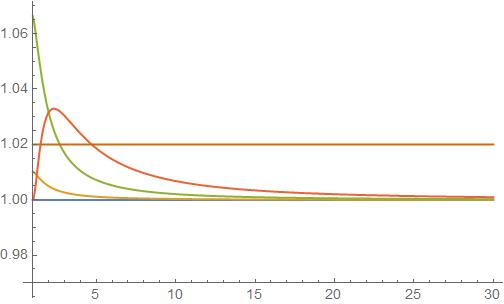
\includegraphics[width = 2\textwidth/3]{images/R^2.jpg}
    \caption{Square distance for various values of $m$ as a function of $\Lambda$, for $k(\Lambda) = \Lambda^2(\Lambda+1)^2$.}
    \label{fig:R2Chi}
\end{figure}

The operator $\chi^1$ has the following symmetric matrix representation
\begin{equation}
    X^\Lambda = \frac{1}{2} 
    \begin{pmatrix} 
    0 & b_\Lambda & 0 & 0& \cdots & 0& 0 & 0 \\
    b_\Lambda & 0 & b_{\Lambda - 1} & 0 & \cdots & 0 & 0 & 0\\
    0 & b_{\Lambda-1} & 0 & b_{\Lambda - 2} & \cdots & 0 & 0 &0\\
    \vdots & \vdots & \ddots & \ddots & \ddots & \vdots & \vdots & \vdots\\
    \vdots & \vdots & \vdots & \ddots & \ddots & \ddots & \vdots & \vdots\\
    \vdots & \vdots & \vdots & \vdots & \ddots & \ddots & \ddots & \vdots\\
    0 & 0 & 0 & 0 & \cdots & b_{2-\Lambda} & 0 & b_{1-\Lambda}\\
    0 & 0 & 0 &0 & \cdots & 0 & b_{1-\Lambda} & 0.
    \end{pmatrix}                                                                                                                           
\end{equation}
in the ordered basis $\{\psi_\Lambda, \psi_{\Lambda - 1}, \dots, \psi_{1-\Lambda}, \psi_{-\Lambda}\}$, where $b_m := \langle \psi_m | \chi^+ | \psi_{m-1} \rangle = \langle \psi_{m-1} | \chi ^- | \psi_m\rangle$ and so
\begin{equation}\label{equationbmD2}
    b_m = \begin{cases}
        \sqrt{1 + \frac{m(m-1)}{k}} + O\left( \frac{m^3}{k^{3/2}} \right), & \text{if } 1- \Lambda \leq m \leq \Lambda \\
        0, & \text{otherwise}.
    \end{cases}
\end{equation}

An additional approximation can be made by replacing the matrix $X^\Lambda$ by $X^\Lambda_0 = \lim_{\Lambda \to \infty} X^\Lambda$, which is the Toeplitz matrix where every nondiagonal entry of $X^\Lambda$ is replaced by a $1$; notice that the smallest value of $b_m$ is $1$ for $m = 0$ and it grows with the absolute value of $m$. Graph \ref{fig:bn} shows the value for the maximum $b_m$ as a function of $\Lambda$ assuming $k(\Lambda) = \Lambda^2(\Lambda+1)^2$. The eigenvectors and their corresponding eigenvalues of the operator $S^1 = \frac{S^+ + S^-}{2}$ represented by $X^\Lambda_0$ are:
\begin{align}
    \tilde \psi_{n} &= \sum_{m = -\Lambda}^\Lambda \sin{\left(\frac{(\Lambda + 1-m)(\Lambda + 1-n)\pi}{2\Lambda + 2}\right)} \psi_m,&
    \tilde \alpha_m &= \cos{\left(\frac{(\Lambda + 1-m)\pi}{2\Lambda + 2}\right)},
\end{align}
each vector with norm $\Lambda + 1$, and with $\tilde \alpha_{\Lambda} > \tilde \alpha_{\Lambda-1} > \cdots > \tilde \alpha_{-\Lambda} $.

\begin{figure}
    \centering
    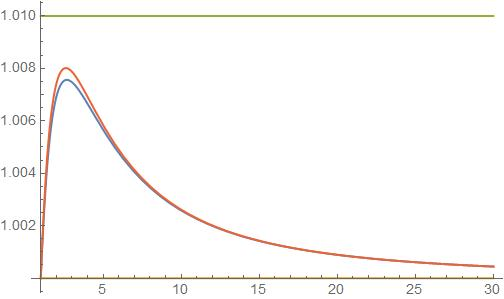
\includegraphics[width = 2\textwidth/3]{images/bn.jpg}
    \caption{Greatest $b_m$ as a function of $\Lambda$, for $k(\Lambda) = \Lambda^2(\Lambda+1)^2$. Red: $b_\Lambda$, Blue: approximation $b_\Lambda \approx \sqrt{1 + \frac{\Lambda(\Lambda - 1)}{k}}$. }
    \label{fig:bn}
\end{figure}

A good estimate, then, of the minimum dispersion is the dispersion of the eigenvector of $S^1$ with maximum absolute value eigenvalue $\tilde \alpha_{\pm \Lambda} = \cos{[\pi/(2\Lambda+2)]}$; in \cite{FioreCoherent2020} it is shown that for this vectors:
\begin{equation}
    (\Delta \vec \chi)^2 < \frac{3.5}{(\Lambda+1)^2} \overset{\Lambda \to \infty}{\longrightarrow} 0.
\end{equation}

The spectrum of $S^1$ satisfies that between any two subsequence eigenvalues in its spectrum for $\Lambda + 1$, $\Lambda_0^{\Lambda + 1}$, there is exactly one in $\Sigma_0^\Lambda$, and, furthermore, $\Sigma_0^\Lambda$ becomes uniformly dense in $[-1, 1]$ as $\Lambda \to \infty$. A similar result \cite{FioreXi2020, FioreTheCase2020} can be obtained for the spectrum of $\chi^1$:
\begin{theorem}
For all $\Lambda \in \NN$, denote the spectrum of $\chi^1$ for $\Lambda$ by $\Sigma^\Lambda_{\chi^1} = \{\alpha_k^\Lambda\}_{n = -\Lambda, \dots, \Lambda }$ ordered in increasing order with $n$. Then:
\begin{enumerate}
    \item If $\alpha$ belongs to $\Sigma^\Lambda_{\chi^1}$, then so does $-\alpha$.
    
    \item $\Sigma_{\Sigma_{\chi^1}}^\Lambda$ and $\Sigma_{\Sigma_{\chi^1}}^{\Lambda+1}$ interlace, i.e. between any two consecutive eigenvalues of $\chi^1$ for $\Lambda +1$, there is exactly one of $\chi^1$ for $\Lambda$:
    \begin{equation}
        \alpha_{\Lambda+1}^{\Lambda+1} > \alpha_{\Lambda}^{\Lambda} > \alpha_\Lambda^{\Lambda+1} > \alpha_{\Lambda-1}^{\Lambda} > \dots > \alpha_{-\Lambda}^{\Lambda} > \alpha_{-\Lambda-1}^{\Lambda+1}.
    \end{equation}
    
    \item $\Sigma_{\chi^1}^\Lambda$ becomes uniformly dense in $[-1, 1]$ as $\Lambda \to \infty$. In particular, $\alpha_{\Lambda}(\Lambda) \geq 1 - \frac{\pi^2}{8(\Lambda + 1)^2}$.
\end{enumerate}
\end{theorem}

In analogy with the study of distances in the fuzzy sphere, we expect this interlacing relation to be useful in the study of the relation between distances for contiguous $\Lambda$'s and for the study of the asymptotic behavior of the distance between this family of vectors.

%Recall that , then they also satisfy the criteria for position observables in $\acal_\Lambda$ given in section \ref{subsectionCriteriaGOodApproximationsOfPosition}, and in fact they also converge uniformly to the operators $e^{\pm i\phi}$ on $L^2(S^1)$ as specified in proposition \ref{theoremConvergesToQMD2}. Taking this definition, the special case in which $\Lambda = 1$ can be studied exactly \cite{FioreCoherent2020}. The eigenvectors of $\chi^1$ are: